\documentclass[12pt]{beamer}
\usepackage[latin1]{inputenc}
\usepackage{fancybox}
\usepackage{soul}
\usepackage{wasysym}
\usecolortheme{wolverine}
\usepackage{graphicx}

\title[]{INF5050 - Protocols and routing in internet}
\subtitle[]{Multiprotocol Label Switching (MPLS) /\newline
			Generalized Multiprotocol Label Switching (GMPLS) }

\author{Khiem-Kim Ho Xuan -- kkho@ifi.uio.no, \newline
		Mattias H�heim Johnsen -- mattiahj@ifi.uio.no}
\date{1. March 2013}
\begin{document}

\begin{frame}
  \titlepage
\end{frame}

\begin{frame}
  \frametitle{Outline}
  \begin{itemize}
  \item Background
  \item MPLS: Fundamentals
  \item MPLS: Terminology
  \item GMPLS
  \item GMPLS: Recovery techniques
  \item Summary
  \item Resources
  \end{itemize}
\end{frame}

\begin{frame}
  \frametitle{Background}

  \begin{itemize}
	\item What is MPLS?
		\begin{itemize}
			\item Mechanism that directs data from one network node to the next based on on path labels rather than network addresses.
			\item MPLS switches packets (IP packets) instead of routing packets to transport the data
		\end{itemize}
	
	\item Why MPLS?
		\begin{itemize}
			\item Provide a highly scalable mechanism that was topology driven rather than flow driven
			\item Load balance traffic to utilize network bandwidth efficiently
			\item Allow core routers/networking devices to switch packets based on a simplified header
			\item Remove the complexity and overhead of network managements (Assemble and reassemble IP packets)
		\end{itemize}			
	\end{itemize} 

  \bigskip

\end{frame}

\begin{frame}
  \frametitle{MPLS was conceived, why?}
  	\begin{itemize}
  		\item The shortest path routing protocols like IS-IS and OSPF
  			\begin{itemize}
  				\item Did not take capacity characteristics into account while
  				making the routing decisions
  				\item The outcome is, segmentation over the network which leads
  				to congestion, while others remain under-utilized.
  			\end{itemize}
  		\item MPLS reduces the complexity and redundancies by adding new network
  		functionalities.
  	\end{itemize}
\end{frame}

\begin{frame}
  \frametitle{MPLS Fundamentals}

  \begin{itemize}
  \item Main idea:
  		\begin{itemize}
  			\item attach a short fixed-length label to packets at the ingress to an MPLS domain
  			\item the labels are used to make the forwarding decisions.
  		\end{itemize}
  	\item MPLS consists of a forwarding and a control plane. Though they are decoupled
  	and independent from each other.
  	\item Supports explicit routed path.
  	\item Provides Quality of Service (QoS) if it is implemented with Diff-Serv and Constraint-based routing.

  \end{itemize}
\end{frame}


\begin{frame}
	\frametitle{Diff-Serv and Constraint-based routing}
		\begin{itemize}
			\item Differentiated Services
				\begin{itemize}
					\item A network architecture for classifying and managing network traffic and provide QoS on modern IP networks.
					\item it is used to provide low-latency to critical network traffic. (Media, VOIP).
				\end{itemize}
			\item Constraint-based routing
				\begin{itemize}
					\item It is a routing technique where resource availability and traffic characterization are taken into account.
				\end{itemize}
		\end{itemize}

\end{frame}

\begin{frame}
	\frametitle{MPLS Fundamentals}
		\begin{figure}[h]
			\begin{center}
				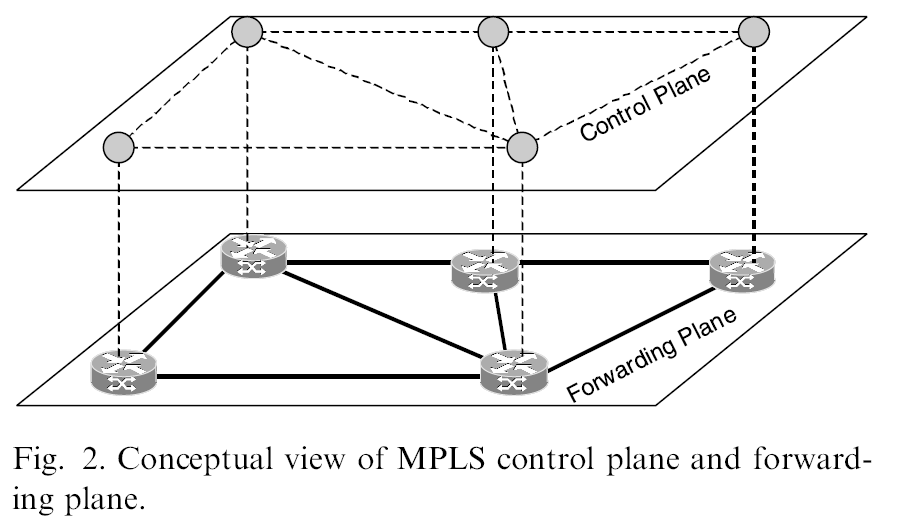
\includegraphics[scale=0.40]{separation.png}
			\end{center}
		\end{figure}
\end{frame}

\begin{frame}
	\frametitle{MPLS Fundamentals: Control Plane}
	
\end{frame}

\begin{frame}
	\frametitle{MPLS Fundamentals: Forwarding Plane}
	
\end{frame}

\begin{frame}
	\frametitle{MPLS architecture}
	
\end{frame}


\begin{frame}
	\frametitle{MPLS: Terminology}
	
	\begin{itemize}
		\item FEC (Forwarding Equivalence Class)
			\begin{itemize}
				\item Group of IP packets which are forwarded in the same manner (e.g. over the same path, with the same priority and the same label)
			\end{itemize}
			
		\item Label
			\begin{itemize}
				\item Short fixed length identifier which is used to identify a FEC
			\end{itemize}						
			
		\item Label Swapping
			\begin{itemize}
				\item Looking up the oncoming label to determine the outgoing label, encapsulation and port
			\end{itemize}
			
		\item Label switched path (LSP)
			\begin{itemize}
				\item Path through one or more LSR for a particular FEC
			\end{itemize}
		\item Label switching router (LSR)
			\begin{itemize}
				\item an MPLS capable router
			\end{itemize}
			
			
	\end{itemize}

\end{frame}

\begin{frame}
	\frametitle{FEC}

	Advantages?	
	\begin{itemize}
		\item 
	\end{itemize}
\end{frame}

\begin{frame}
\frametitle{Disadvantages of MPLS}
	
\end{frame}





\begin{frame}
  \frametitle{GMPLS}

  \begin{itemize}
  \item What is GMPLS?
  	\begin{itemize}
  		\item  a protocol suite extending MPLS to manage further classes of interfaces and switching technologies other than packet interfaces and switching, such as time division multiplex, layer-2 switch, wavelength switch and fiber-switch.
  	\end{itemize}
  \end{itemize}
\end{frame}

\begin{frame}
	\frametitle{GMPLS}
	\begin{itemize}
	

	  		\item GMPLS is an extended form of MPLS and some of these improvements are:
			\begin{itemize}
				\item RSVP-TE
				\item OSPF and IS-IS
				\item New link-management protocol
				\item Bi-directional LSP setup
					\begin{itemize}
						\item Reduce latency
						\item Less control overhead
						\item Route selection is simpler
						\item Cleaner interface
					\end{itemize}									
			\item MPLS emphasizes the seperation of control plane and network plane
			\item GMPLS extends this seperation and allows the control plane to be physically diverse from the associated data plane
				
			\end{itemize}		
				\end{itemize}
\end{frame}

\begin{frame}
  \frametitle{GMPLS: Hierarchial LSP}

  \begin{itemize}
  \item 
    %\pause
  \item 
  \end{itemize}
\end{frame}




\begin{frame}
  \frametitle{Summary}
  \begin{itemize}
  \item MPLS
    %\pause
  \item GMPLS
  \end{itemize}
\end{frame}

\begin{frame}
  \frametitle{Resources}
  \begin{itemize}
  \item Generalized Multiprotocol Label Switching: An Overview of Signaling Enhancements and Recovery Techniques
IEEE Communication Magazine, July 2001.
A. Banerjee et. al. 
  \item Internet Traffic Engineering Using Multi-Protocol Label Switching (MPLS).
Computer Networks 40, Elsevier, 2002
D.O. Awduche and B. Jabbari. 
  \end{itemize}
\end{frame}

\end{document}
